\documentclass[tikz,border=10pt,12pt]{standalone}
% Shared preamble for standalone-compiled dc_paper figures.
% Copies just the bits of dc_paper.tex's preamble that figures need.

\usepackage{amsmath,amssymb,amsthm,mathtools,bm}
\usepackage{siunitx}
\sisetup{detect-all,group-separator={,},per-mode=symbol}

\usepackage[T1]{fontenc}
\usepackage{xcolor}
\usepackage{enumitem}
\usepackage{mathpazo}                % Palatino body + matching math
\usepackage[scaled=0.92]{helvet}     % Helvetica sans
\usepackage{courier}                 % monospace
\usepackage{microtype}

% --- IA brand colour palette (must match dc_paper.tex) ---
\definecolor{iadark}{HTML}{1B1815}
\definecolor{iabone}{HTML}{FAFAF7}
\definecolor{iaaccent}{HTML}{A04A1F}
\definecolor{iataupe}{HTML}{F2EDE6}
\definecolor{iarule}{HTML}{3A332D}
\definecolor{iagrey}{HTML}{5A524A}

% --- graphics ---
\usepackage{tikz}
\usepackage{circuitikz}
\usepackage{pgfplots}
\pgfplotsset{compat=1.18}
\usetikzlibrary{arrows.meta,positioning,shapes.geometric,calc,fit,
                decorations.pathreplacing,decorations.markings,
                shadows.blur,backgrounds}

% --- math macros from dc_paper.tex preamble (figures use them) ---
\newcommand{\E}{\mathbb{E}}
\newcommand{\Var}{\operatorname{Var}}
\newcommand{\Cov}{\operatorname{Cov}}
\newcommand{\Cor}{\operatorname{Cor}}
\newcommand{\Prb}{\mathbb{P}}
\newcommand{\R}{\mathbb{R}}
\newcommand{\N}{\mathbb{N}}
\newcommand{\1}{\mathbf{1}}
\newcommand{\VaR}{\operatorname{VaR}}
\newcommand{\TVaR}{\operatorname{TVaR}}
\newcommand{\ES}{\operatorname{ES}}
\newcommand{\dd}{\mathrm{d}}
\newcommand{\given}{\,\vert\,}
\newcommand{\set}[1]{\left\{#1\right\}}
\newcommand{\norm}[1]{\left\Vert #1 \right\Vert}
\DeclareMathOperator*{\argmin}{arg\,min}
\DeclareMathOperator*{\argmax}{arg\,max}

% \textwidth has no meaning in standalone class; give it a value matching
% the paper's A4 + 1-inch margins so any leftover \resizebox{\textwidth}
% gracefully sizes the figure to that nominal width.
\setlength{\textwidth}{15.92cm}

\begin{document}
\pagecolor{iabone}
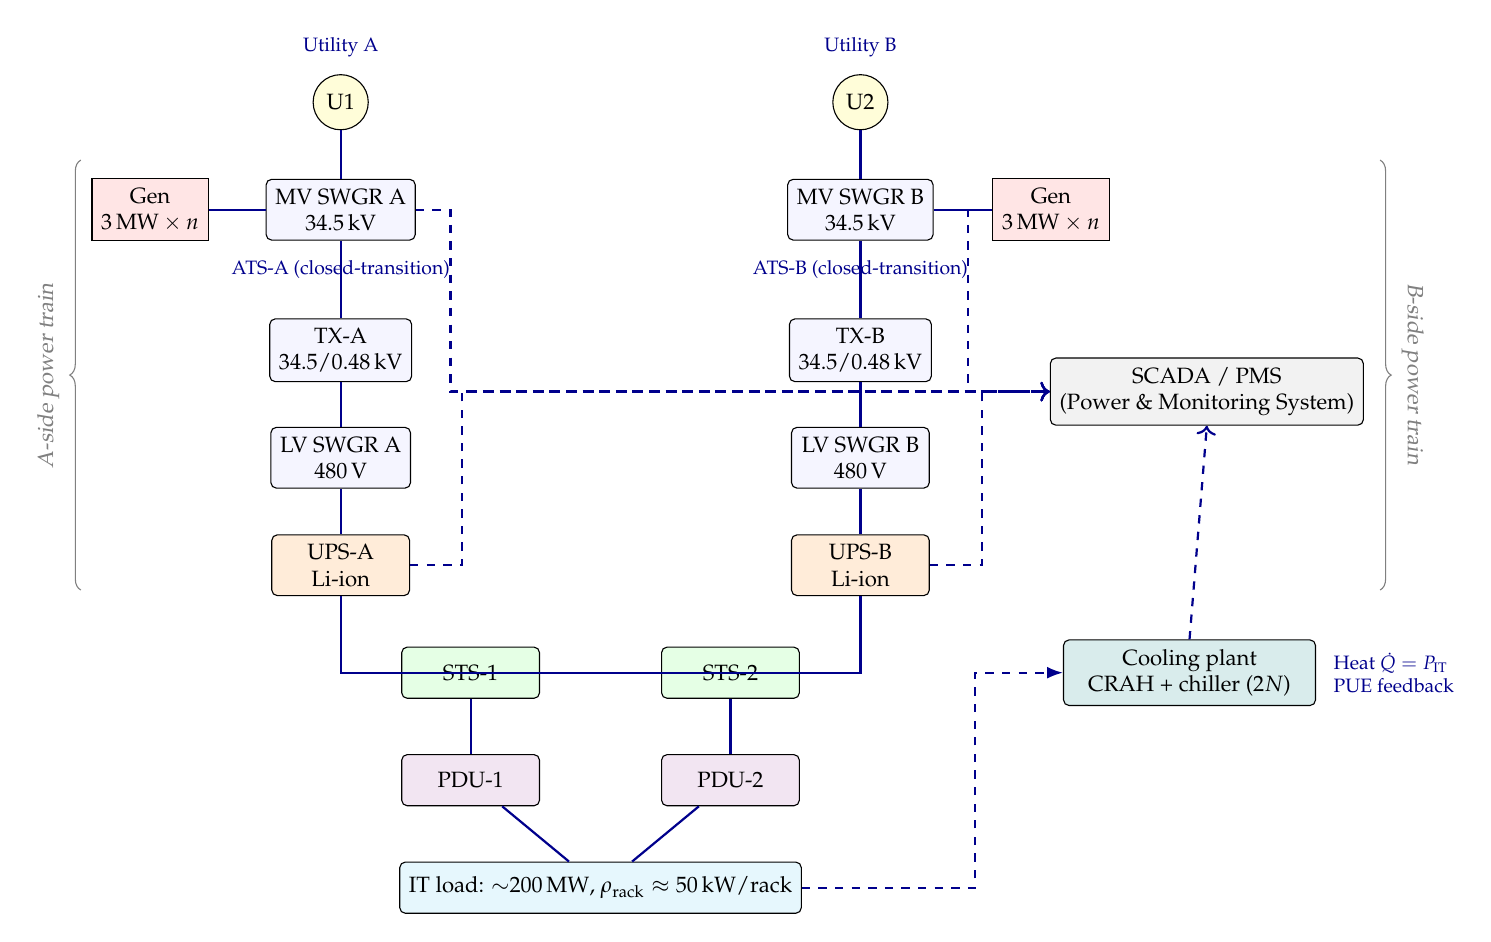
\begin{tikzpicture}[
    every node/.style={font=\footnotesize},
    blk/.style={draw,rounded corners=2pt,minimum width=1.75cm,minimum height=0.65cm,
                align=center,fill=blue!4},
    src/.style={draw,circle,minimum size=0.7cm,inner sep=0pt,fill=yellow!15},
    gen/.style={draw,rectangle,minimum width=1.15cm,minimum height=0.65cm,fill=red!10,align=center},
    bus/.style={draw,line width=1.2pt,blue!55!black},
    line/.style={-{Latex[length=2mm]},thick,blue!55!black},
    fline/.style={thick,blue!55!black},
    label/.style={font=\scriptsize,blue!55!black},
    x=1.1cm, y=1.05cm
]

% Utility side
\node[src] (U1) at (0,9) {U1};
\node[src] (U2) at (6,9) {U2};
\node[label,above=0.10cm of U1] {Utility A};
\node[label,above=0.10cm of U2] {Utility B};

% MV switchgear
\node[blk] (MVA) at (0,7.7) {MV SWGR A\\\SI{34.5}{\kilo\volt}};
\node[blk] (MVB) at (6,7.7) {MV SWGR B\\\SI{34.5}{\kilo\volt}};

\draw[fline] (U1) -- (MVA);
\draw[fline] (U2) -- (MVB);

% Generators / ATS
\node[gen] (G1) at (-2.2,7.7) {Gen\\ $3\,\mathrm{MW}\times n$};
\node[gen] (G2) at ( 8.2,7.7) {Gen\\ $3\,\mathrm{MW}\times n$};
\draw[fline] (G1) -- (MVA);
\draw[fline] (G2) -- (MVB);

% ATS labels
\node[label,below=0.12cm of MVA] {ATS-A (closed-transition)};
\node[label,below=0.12cm of MVB] {ATS-B (closed-transition)};

% Step-down transformers
\node[blk] (TXA) at (0,6.0) {TX-A\\$34.5/0.48$\,kV};
\node[blk] (TXB) at (6,6.0) {TX-B\\$34.5/0.48$\,kV};
\draw[fline] (MVA) -- (TXA);
\draw[fline] (MVB) -- (TXB);

% LV switchgear
\node[blk] (LVA) at (0,4.7) {LV SWGR A\\480\,V};
\node[blk] (LVB) at (6,4.7) {LV SWGR B\\480\,V};
\draw[fline] (TXA) -- (LVA);
\draw[fline] (TXB) -- (LVB);

% UPS modules
\node[blk,fill=orange!15] (UA) at (0,3.4) {UPS-A\\Li-ion};
\node[blk,fill=orange!15] (UB) at (6,3.4) {UPS-B\\Li-ion};
\draw[fline] (LVA) -- (UA);
\draw[fline] (LVB) -- (UB);

% Static transfer switches
\node[blk,fill=green!10] (STSA) at (1.5,2.1) {STS-1};
\node[blk,fill=green!10] (STSB) at (4.5,2.1) {STS-2};
\draw[fline] (UA) |- (STSA);
\draw[fline] (UB) |- (STSA);
\draw[fline] (UA) |- (STSB);
\draw[fline] (UB) |- (STSB);

% PDUs
\node[blk,fill=violet!10] (PD1) at (1.5,0.8) {PDU-1};
\node[blk,fill=violet!10] (PD2) at (4.5,0.8) {PDU-2};
\draw[fline] (STSA) -- (PD1);
\draw[fline] (STSB) -- (PD2);

% Rack loads
\node[blk,fill=cyan!10,minimum width=4.2cm] (LOAD) at (3,-0.5)
    {IT load: $\sim$\SI{200}{MW}, $\rho_{\mathrm{rack}}\approx\SI{50}{\kilo\watt\per rack}$};
\draw[fline] (PD1) -- (LOAD);
\draw[fline] (PD2) -- (LOAD);

% Cooling plant
\node[blk,fill=teal!15,minimum width=3.2cm] (COOL) at (9.8,2.1)
    {Cooling plant\\CRAH + chiller ($2N$)};
\draw[line,dashed] (LOAD.east) -- ++(2,0) |- (COOL);
\node[label,right=0.1cm of COOL,align=left]
    {Heat $\dot Q = P_{\mathrm{IT}}$\\PUE feedback};

% PMS / SCADA box — narrowed slightly and aimed at .west so the SCADA
% dashed lines enter cleanly on the left edge instead of plunging into
% the centre of the box.
\node[blk,fill=gray!10,minimum width=3.0cm] (PMS) at (10.0,5.5)
    {SCADA / PMS\\(Power \& Monitoring System)};
\draw[line,dashed,->] (MVA.east) -- ++(0.4,0) |- (PMS.west);
\draw[line,dashed,->] (MVB.east) -- ++(0.4,0) |- (PMS.west);
\draw[line,dashed,->] (UA.east) -- ++(0.6,0) |- (PMS.west);
\draw[line,dashed,->] (UB.east) -- ++(0.6,0) |- (PMS.west);
\draw[line,dashed,->] (COOL.north) -- (PMS.south);

% Bracket: "A side" / "B side"
% A-side brace stays at x=-3 (plenty of free space on the left).
% B-side brace moved out to x=12 so it sits clear of the SCADA box
% (whose east edge is at x=11.5). Previously the brace ran straight
% through the middle of SCADA and the rotated label fell ON TOP of it.
\draw[decorate,decoration={brace,amplitude=4pt,mirror},gray]
   (-3,8.3) -- (-3,3.1) node[midway,left=0.15cm,rotate=90,anchor=south]
   {\textsl{A-side power train}};
\draw[decorate,decoration={brace,amplitude=4pt},gray]
   (12.0,8.3) -- (12.0,3.1) node[midway,right=0.15cm,rotate=-90,anchor=south]
   {\textsl{B-side power train}};

\end{tikzpicture}%
\end{document}
